\documentclass{article}
\usepackage[utf8]{inputenc}
\usepackage[T1]{fontenc}
\usepackage[dvipsnames]{xcolor}
\usepackage{color}
\usepackage{colortbl}
\usepackage{enumitem}
\usepackage{tgbonum}
\usepackage[english]{babel}
\usepackage[a4paper,top=2cm,bottom=2cm,left=3cm,right=3cm,marginparwidth=1.75cm]{geometry}
\usepackage{graphicx} % Required for inserting images
\usepackage{amsmath}

\usepackage{caption}
\usepackage{lipsum}

\title{Challenge 1}
\author{Agolli Raul, Guaiumi Gioele}
\date{October 2025}

\begin{document}
\maketitle

\section{Experimental Setup}

\begin{itemize}
    \item \textbf{Language}: C++, Python (Google Colab environment)
    \item \textbf{Libraries}:
        \begin{itemize}
            \item \textbf{boost::multiprecision} for big integers (512/1024 bit)
            \item \textbf{boost::random} for random base selection
            \item \textbf{google/benchmark} for measuring asymptotic runtime
            \item \textbf{matplotlib} to plot the benchmark results
        \end{itemize}
    \item \textbf{Inputs}: 512-bit primes and generated random numbers
\end{itemize}

\section{Algorithm Description \& Design Choices}
\begin{itemize}
    \item Based on the algorithm from the lecture
    \item Single-round modular exponentiation: \textbf{power(a, n-1, n)} with detection of non-trivial square roots of 1
    \item Utilized multiprecision types provided by \textbf{boost} library to handle 512-bit numbers
\end{itemize}

\section{Benchmark \& Performance}
\begin{itemize}
    \item \textbf{Asymptotic behavior}: Expected $O(log^2(n) log(p))$ due to repeated modular multiplications in exponentiation
    \item \textbf{Observed behavior}: Because the Google Benchmark library cannot directly handle arbitrarily large integers, we used the exponent of the number as the benchmark input instead of the full integer value. 
    
    In practice, this means that instead of testing with values like $2^k$ directly, the benchmark receives $k$ as parameter. This transforms the input scale into a logarithmic domain, so the complexity reported by the benchmark is expressed in terms of the exponent rather than the actual integer size. As a consequence, the automated benchmark reports a complexity of $O(n^2)$.
    
    We observed a strong match between the theoretical complexity and our experimental measurements using the Matplotlib library. In the figure below (logarithmic scale), the blue curve shows the measured performance, while the orange curve represents the theoretical reference. Each experimental point corresponds to the average of 5 runs for the same input, along with its standard deviation. The theoretical complexity was modeled as the cube of the input (equivalent to $log^3n$ on a linear scale), multiplied by a constant factor that we determined experimentally.
\end{itemize}

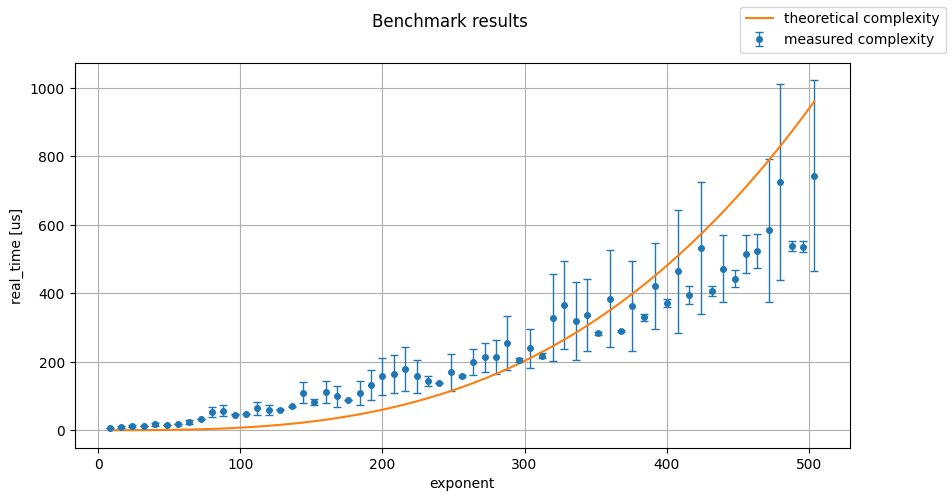
\includegraphics[width=\linewidth]{benchmark-plot-3.png}

\section{Validation \& Testing}

To verify both the correctness and reliability of our primality-testing implementation, we performed two complementary experiments:

\begin{itemize}
    \item \textbf{Validation with Known Large Primes (test.cpp)} comparison over 20 random numbers:

    We tested the algorithm using a fixed list of 512-bit primes.
    For each number:
    \begin{itemize}
        \item The algorithm was executed up to \textbf{25 independent trials}.
        \item If the function returned “composite” at any iteration, the test immediately reported a failure.
        \item Otherwise, the number was classified as “probably prime”.
    \end{itemize}
    
    \item \textbf{Statistical Accuracy Evaluation (test2.cpp)}
    
    To assess the probability of correctness across multiple confidence levels, we ran an extensive randomized test:
    \begin{itemize}
        \item \textbf{100 random integers} between 2 and 10,000 were generated.
        \item For each number, the Boost Miller–Rabin implementation (25 rounds) was used as a \textbf{trusted reference}. 25 trials was chosen because it guarantees an error of around $0.25^{25}$ on the worst case.
        \item Our custom algorithm was tested with \textbf{1, 5, 10, and 25 repetitions}.
        \item Each configuration (1/5/10/25 trials\footnote{each configuration correspond to a level confidence (w.r.t. the worst case) of $1-0.25^{trials}$}) was repeated \textbf{2000 times per input}, recording whether the result matched the Boost baseline.
    \end{itemize}
    For each number, we computed:
    \begin{itemize}
        \item The \textbf{mean correctness rate} for each confidence level.
        \item A final summary table showing:
        \begin{itemize}
            \item The tested number
            \item Ground truth primality (from Boost)
            \item Accuracy for 1, 5, 10, and 25 trials
        \end{itemize}

        This experiment quantifies how the error probability decreases as the number of iterations increases, and confirms that the expected probabilistic guarantees hold in practice.
        
    \end{itemize}
\end{itemize}
%add ercentuale di confidenza dei risultati rispetto al worst case
\end{document}
